\documentclass[]{uniqueness_cv}

\titleformat{\section}[block]{\Large\scshape\raggedright}{}{0em}{}[\color{blue}{\titlerule[2pt]}]
\titlespacing{\section}{5pt}{3pt}{7pt}

\newcommand*\arc{{\fontfamily{pbk}\fontseries{db}\selectfont+}}

\begin{document}

%%%%%%%%%%%%%%%%%%%%%%%%%%%%%%%%%%%%%%
%
%     LAST UPDATED DATE
%
%%%%%%%%%%%%%%%%%%%%%%%%%%%%%%%%%%%%%%
\lastupdated

%%%%%%%%%%%%%%%%%%%%%%%%%%%%%%%%%%%%%%
%
%     TITLE NAME
%
%%%%%%%%%%%%%%%%%%%%%%%%%%%%%%%%%%%%%%

\header{Debarghya}{Das}
       {social network analyst}
\namesection{akshay}{koli}{
\urlstyle{same}\url{http://akshaykoli.com} \\
\phone   {+1~(234)~567~890}\\
\Mobilefone   {8586825185}\\
\Email{\href{mailto:akoli0082@gmail.com}{akoli0082@gmail.com}}\\
\href{mailto:dd367@cornell.edu}{dd367@cornell.edu} | 607.379.5733}

\vspace{15pt}

\section{\textcolor{gray}{\ding{58}} About Me}
 This is another paragraph, contains some text to test the paragraph interlining, paragraph indentation and some other features. Also, is easy to see how new paragraphs are defined by simply entering a double blank space.This is another paragraph,Lorem.
This is another paragraph, contains some text to test the paragraph interlining, paragraph indentation and some other features latex.

%%%%%%%%%%%%%%%%%%%%%%%%%%%%%%%%%%%%%%
%
%     COLUMN ONE
%
%%%%%%%%%%%%%%%%%%%%%%%%%%%%%%%%%%%%%%

\begin{minipage}[t]{0.33\textwidth} 

%%%%%%%%%%%%%%%%%%%%%%%%%%%%%%%%%%%%%%
%     EDUCATION
%%%%%%%%%%%%%%%%%%%%%%%%%%%%%%%%%%%%%%

\section{ \textcolor{gray}{\ding{58}} Education} 

\subsection{Cornell University}
\descript{MEng in Computer Science}
\location{Expected Dec 2014 | Ithaca, NY \\ Cum. GPA: N/A}
\sectionsep


\descript{BS in Computer Science}
\location{Expected May 2014 | Ithaca, NY}
Conc. in Software Engineering \\
College of Engineering \\
Dean's List (All Semesters) \\
\location{ Cum. GPA: 3.92 / 4.0 \\
Major GPA: 3.94 / 4.0}
\sectionsep

%%%%%%%%%%%%%%%%%%%%%%%%%%%%%%%%%%%%%%
%     SKILLS
%%%%%%%%%%%%%%%%%%%%%%%%%%%%%%%%%%%%%%

\section{ \textcolor{gray}{\ding{58}} Programming Skills}

\includegraphics[scale=0.80]{img/5stars.png}\\
Java \textbullet{}   Shell \textbullet{} JavaScript \textbullet{} Matlab \\
OCaml\textbullet{}Python\textbullet{}Rails\textbullet{}\LaTeX\ \\

\includegraphics[scale=0.80]{img/4stars.png}\\
C \textbullet{} C++ \textbullet{} CSS \textbullet{} PHP \textbullet{} Assembly \\

\includegraphics[scale=0.80]{img/2stars.png}\\
AS3 \textbullet{} iOS \textbullet{} Android \textbullet{} MySQL
\sectionsep

\section{ \textcolor{gray}{\ding{58}} Personal Skills}
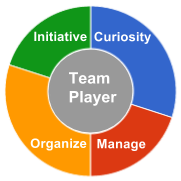
\includegraphics[scale=0.80]{img/personal.png}\\
\sectionsep

\end{minipage}
\hfill
\begin{minipage}[t]{0.66\textwidth} 

%%%%%%%%%%%%%%%%%%%%%%%%%%%%%%%%%%%%%%
%     EXPERIENCE
%%%%%%%%%%%%%%%%%%%%%%%%%%%%%%%%%%%%%%

\section{ \textcolor{gray}{\ding{58}} Experience}

\runsubsection{Coursera}
\descript{| KPCB Fellow + Software Engineering Intern }
\location{Expected June 2014 – Sep 2014 | Mountain View, CA}
\vspace{\topsep} % Hacky fix for awkward extra vertical space
\begin{tightemize}\item 52 out of 2500 applicants chosen to be a KPCB Fellow 2014.
\end{tightemize}
\sectionsep

\runsubsection{Google}
\descript{| Software Engineering Intern }
\location{May 2013 – Aug 2013 | Mountain View, CA}
\begin{tightemize}
\item Worked on the YouTube Captions team in primarily vanilla Javascript and Python to plan, design and develop the full stack implementation of a new framework to add and edit Automatic Speech Recognition captions.\item Created a backbone.js-like framework for the Captions editor.\item All code was reviewed, perfected, and pushed to production.\end{tightemize}
\sectionsep
%%%%%%%%%%%%%%%%%%%%%%%%%%%%%%%%%%%%%%
%     RESEARCH
%%%%%%%%%%%%%%%%%%%%%%%%%%%%%%%%%%%%%%
\section{ \textcolor{gray}{\ding{58}} Application Developed}
\begin{tabular}{r|p{11cm}}
\runsubsection{\textsc{Fab'2015} & \textsc{Antardhvani Android App}}\\&\footnotesize{The Delhi University Antardhvani Cultural Festival was conceptualized and started in 2011 and has become the showpiece event of India’s highest rated university.The annual Cultural Festival of the University of Delhi was named ’Antardhvani’ by Vice Chancellor.
Link : https://play.google.com/store/apps/details?id=antardhvani.du.ac.in.antardhvani.}\\\\
\runsubsection{\textsc{Nov'2014} & \textsc{Mini-shell}}\\&\footnotesize{This is a mini-UNIX-shell (a simple mini-Unix-Shell written in C). It employs system calls to execute the commands. Many trivial functions of shell has been incorporated in it   .
Link : https://github.com/akki12345/Mini-Awesome-Shell}\\\\
\runsubsection{\textsc{dec'2014} & \textsc{Travelling Salesman Problem And Hamiltonian Cycle}}\\&\footnotesize{Travelling Salesman Problem (TSP): Given a set of cities and distance between every pair of cities,the problem is to find the shortest possible route that visits every city exactly once and returns to the starting point.}
\\&\footnotesize{Link : https://github.com/akki12345/Travelling-SalesMan-problem.}
\\&\footnotesize{Hamiltonian Cycle: A Hamiltonian cycle, also called a Hamiltonian circuit, is a graph cycle (i.e., closed loop) through a graph that visits each node exactly once.Design algorihtm and implement in C lan
guage.}
\\&\footnotesize{Link :https://github.com/akki12345/Detect-Hamiltonian-cycle-in-Graph-.}\\\\
\runsubsection{\textsc{Nov'2014} & \textsc{Mini-shell}}\\&\footnotesize{This is a mini-UNIX-shell (a simple mini-Unix-Shell written in C). It employs system calls to execute the commands. Many trivial functions of shell has been incorporated in it   .
Link : https://github.com/akki12345/Mini-Awesome-Shell}\\\\
\end{tabular}

\end{minipage}
\end{document}  
\documentclass[]{article}
